%%%%%Präambel%%%%%

\documentclass[12pt,a4paper]{article}%Schriftgröße, Papierformat einstellen
%\documentclass{scrbook}
\usepackage[top=30mm,bottom=30mm]{geometry}
\usepackage{lipsum}
%Pakete laden zur deutschen Rechtschreibung und für Umlaute
\usepackage[T1]{fontenc}
\usepackage[ngerman]{babel}
\usepackage[utf8]{inputenc} %für Windows, Linux
%\usepackage[applemac]{inputenc} %für Mac
%\usepackage{xcolor}
\usepackage{graphicx}
\usepackage[dvipsnames]{xcolor} %provides more easily callable colors
\usepackage{cancel} %needed to cancel letters
\usepackage{titlesec} %this package is needed to make the \subsubsubsection{} personal section
\usepackage{cite} %for citation
\usepackage{filecontents} %enables this to generate external files. I dunno where i needed this
\usepackage{tabularx} %to make tabulars with fixed width
\usepackage{harvard} %for harvard citation
\usepackage{units} %to call units
\usepackage{longtable} %to make tables over multiple pages
\usepackage{chngcntr} %forgot what this is but too scared to delete it
\usepackage{stmaryrd} %forgot what this is but too scared to delete it
\usepackage{array} %kinda similar to a tabular, used to make vectors
\let\harvardleftorig\harvardleft
%\usepackage[round]{natbib}
%\usepackage{hyperref}
\usepackage[nottoc,numbib]{tocbibind}

%Pakete laden zu mathematischen Symbolen etc.
\usepackage{calc} 
\usepackage{amsmath,amssymb,amsthm}
%Make headings and footings
\usepackage{scrpage2}
\pagestyle{scrheadings}
\clearscrheadfoot
\automark[chapter]{section}
\ofoot{\pagemark}
\ifoot{Florian Leuze}
\chead{\headmark}
\setfootsepline{1pt}
\setheadsepline{1pt}
%\setheadsepline[\textwidth+20pt]{0.5pt}

%Inhaltsverzeichnis mit Links erstellen
\usepackage[colorlinks,
pdfpagelabels,
pdfstartview = FitH,
bookmarksopen = true,
bookmarksnumbered = true,
linkcolor = black,
plainpages = false,
hypertexnames = false,
citecolor = black] {hyperref}

% Umgebungen für Definitionen, Sätze, usw.
\newtheorem{satz}{Satz}[section]
\newtheorem{definition}[satz]{Definition}     
\newtheorem{lemma}[satz]{Lemma}	
% Es werden Sätze, Definitionen etc innerhalb einer Section mit
% 1.1, 1.2 etc durchnummeriert, ebenso die Gleichungen mit (1.1), (1.2) ..                  
\numberwithin{equation}{section}

\setcounter{secnumdepth}{4} %Has something to do with index

%generating everything needed for subsubsubsection
\titleformat{\paragraph}
{\normalfont\normalsize\bfseries}{\theparagraph}{1em}{}
\titlespacing*{\paragraph}
{0pt}{3.25ex plus 1ex minus .2ex}{1.5ex plus .2ex}

%Shortcuts for number ranges
\newcommand{\R}{\mathbb{R}} %zB \R als Abkürzung für das Symbol der reellen Zahlen
\newcommand{\N}{\mathbb{N}}
\newcommand{\Z}{\mathbb{Z}}
\newcommand{\Q}{\mathbb{Q}}
\newcommand{\C}{\mathbb{C}}

%defining the command for subsubsubsection
\newcommand{\subsubsubsection}{\paragraph}

%command to cite like: blabla (vgl. ...)
\newcommand\citevgl
{\def\harvardleft{(vgl.\ \global\let\harvardleft\harvardleftorig}%
 \cite
}

%command to cite like: blablabla. (Vgl. ...)
\newcommand\citeVgl
{\def\harvardleft{(Vgl.\ \global\let\harvardleft\harvardleftorig}%
 \cite
}

%Define easy functions for colors
\def\colBord#1{\begingroup\color{Fuchsia}{#1}\endgroup}
\def\colRed#1{\begingroup\color{Red}{#1}\endgroup}
\def\colGreen#1{\begingroup\color{LimeGreen}{#1}\endgroup}
\def\colBlue#1{\begingroup\color{NavyBlue}{#1}\endgroup}

%define easy function to underset directly with a color
\def\usGreen#1#2{\underset{\colGreen{#1}}{#2}}
\def\usBord#1#2{\underset{\colBord{#1}}{#2}}

%define easy functions to underbrace directly with a color
\def\ubGreen#1#2{\underbrace{#2}_{\colGreen{#1}}}

%function for fat def
\def\defF{\textbf{Def.: }}

%vecT generates an array, vecD generates an array with dotts in the middle
\def\vecT#1{\left(\begin{array}{c} #1 \end{array}\right)}
\def\vecD#1{\vecT{#1_1 \\ \dddot \\ #1_d}}

%just generates three dots. Useful for n dimensional vectors and matrixes
\def\dddot{\cdot \\ \cdot \\ \cdot}

%Use this if you have a tabular but want to summarize 2 or 3 cells
%#1 is the argument for the table type (r, l, c, X, you can also ad | |)
%#2 is the text in the cell
\def\multiTwo#1#2{\multicolumn{2}{>{\hsize=\dimexpr2\hsize+2\tabcolsep+\arrayrulewidth\relax}#1}{#2}}
\def\multiThree#1#2{\multicolumn{3}{>{\hsize=\dimexpr3\hsize+4\tabcolsep+2\arrayrulewidth\relax}#1}{#2}}

%it will write element of R just to make things more easy
\def\inR#1{\qquad ,\; #1 \in \R}

%will put everything in #1 in bracks (with proper height)
\def\bracks#1{\left[ #1 \right]}

%this is needed to make fixed size cells where you can adjust the orientation.
%if you need just copy and do a raggedcenter
\newcolumntype{L}[1]{>{\raggedleft\let\newline\\\arraybackslash\hspace{0pt}}m{#1}}
\newcolumntype{R}[1]{>{\raggedright\let\newline\\\arraybackslash\hspace{0pt}}m{#1}}

\def\equate#1{$#1$}

%Useful function if you do a formula colletion. 
%#1 Name of the Formula
%#2 formula, you dont need maths mode
\def\formTab#1#2{
\begin{equation}
  \begin{tabularx}{12cm}{R{3cm} l l}
    #1 &: &$#2$
  \end{tabularx}
\end{equation}
}

%exactly the same as formTab but this will also generate a label which you will be able to call
%#1 Name of the Formula
%#2 formula, you dont need maths mode
%#3 Name of the label. Attention, identifier "eq:" will be added automatically
\newcommand{\formTabL}[3]{
\begin{equation}
  \begin{tabularx}{12cm}{R{3cm} l l}
    #1 &: &$#2$ 
  \end{tabularx}
  \label{eq:#3}
\end{equation}}


%\setlength\abovedisplayskip{0pt}

% Auf der Seite http://detexify.kirelabs.org/classify.html können Sie mathematische Symbole, Pfeile usw per Maus eingeben und bekommen den Latex-Befehl dafür angezeigt.
% detexify gibt es auch als App...

%jetzt beginnt das eigentliche Dokument
\begin{document}
\bibliographystyle{agsm}

\author{}
\title{\underline{Elektro F} \\ $\;$ \\ \underline{Grundlagen der Elektrotechnik} \\ $\;$ \\ $\;$ \\ Florian Leuze}
\date{}

\maketitle % erzeugt den Kopf
\newpage
\section{\underline{Inhalt}}
\tableofcontents

\subsection{Versionierung}
\begin{tabular}{|p{2cm}|p{1cm}|p{1.5cm}|p{8.5cm}|}\hline
Datum & Vers. & Kürzel & Änderung \\ \hline
26.04.2018 & 0.1 & FL & Erzeugung Dokument; Erzeugung Inhaltsverzeichnis; Erzeugung Versionierung; Erzeugung Literaturverzeichnis; 
Erzeugung 2.1 - 2.3.2; 3.1 - 3.4.1 \\ \hline
27.04.2018 & 0.1 & FL & Erzeugung 3.5 - 3.7.1; Erzeugung  \\ \hline
28.04.2018 & 0.1 & FL & Erzeugung 4 - 4.2.5; Erzeugung 2.3.3 - 2.3.4; Erweiterung 5.1; Neuimplementierung 5.1 mit longtable \\ \hline
07.05.2018 & 0.1 & FL & Erzeugung Elektrische Quellen; Systematische Verfahren zur Netzwerkanalyse - Knotenspannungsanalyse \\ \hline
\end{tabular}

\newpage
 
\section{\underline{Grundlagen}}
\subsection{SI-Basiseinheiten}
\begin{tabular} {|c|c|c|}\hline
Bezeichnung & Einheit & Bedeutung \\ \hline
Meter & m & Einnheit der Länge \\ \hline
Kilogramm & kg & Einheit der Masse \\ \hline
Sekunde & s & Einheit der Zeit \\ \hline
Ampere & A & Eineit der Stromstärke \\ \hline
Kelvin & K & Einheit der Temperatur \\ \hline
Mol & mol & Einheit der Stoffmenge \\ \hline
Candela & cd & Einheit der Lichtstärke \\ \hline
\end{tabular}

\subsection{Vorsatzzeichen}
\begin{tabular} {|c|c|c|c|c|c|} \hline
Name & Zeichen & Zehnerpotenz & Name & Zeichen & Zehnerpotenz \\ \hline
Yotta & Y & $10^{24}$ & Dezi & d & $10^{-1}$ \\ \hline
Zetta & Z & $10^{21}$ & Centi & c & $10^{-2}$ \\ \hline
Exa & E & $10^{18}$ & Milli & m & $10^{-3}$ \\ \hline
Peta & P & $10^{15}$ & Mikro & $\mu$ & $10^{-6}$ \\ \hline
Tera & T & $10^{12}$ & Nano & n & $10^{-9}$ \\ \hline
Giga & G & $10^{9}$ & Piko & p & $10^{-12}$ \\ \hline
Mega & M & $10^{6}$ & Femto & f & $10^{-15}$ \\ \hline
Kilo & k & $10^{3}$ & Atto & a & $10^{-18}$ \\ \hline
Hekto & h & $10^{2}$ & Zepto & z & $10^{-21}$ \\ \hline
Deka & da & $10^{1}$ & Yokto & y & $10^{-24}$ \\ \hline
\end{tabular}

\subsection{Misc}
\subsubsection{Atome}
\begin{itemize}
\item Atome sind im Grundzustand neutral
\item Ändert sich die Zahl der Elektronen spricht man von Ionisierung:
\begin{itemize}
\item positives Ion = Kation (weniger Elektronen)
\item negatives ion = Anion (mehr Elektronen)
\end{itemize}
\item Elektron $q_e = -e$, Elektronenmasse: $m_e = 9,109... * 10^{-31}kg$ 
\item Proton $q_p = +e$, Protonenmasse: $m_p = 1,672... * 10^{-27}kg$
\end{itemize}

\subsubsection{Konstanten}
\begin{tabular} {|p{2cm}|p{4cm}|p{1.5cm}|p{5.5cm}|} \hline
Bezeichner & Wert & Einheit & Bedeutung \\ \hline
\rule{0pt}{15pt}
$\varepsilon_0$ & $8,854... * 10^{-12}$ & $\frac{As}{Vm}$ & Dielektrizitätskonstante des Vakuums \\ \hline
$e$ & $1,602176... * 10^{-19}$ & $C$ & Elementarladung \\ \hline
\end{tabular}

\subsubsection{Spezifische Widerstände $\left[\mu \Omega cm \right]$}
\begin{tabularx}{14.7cm}{|X|X|X|X|X|X|}\hline
Cu & Au & Ag & Al & Cr & Ta \\ \hline
$1,673$ & $2,35$ & $1,59$ & $2,655$ & $14,1$ & $13,5$ \\ \hline
\end{tabularx}

\subsubsection{Temperaturkoeffizienten $\alpha$ ohmscher Widerstände bei $20^{\circ} C$ in $\left[\frac{1}{^{\circ} C} \right]$}
\begin{tabularx}{14.7cm}{|X|X|X|X|X|X|X|} \hline
Cu & Ag & Au & Al & Ta & Ni & Konst. \\ \hline
$3,9 * 10^{-3}$ & $3,8 * 10^{-3}$ & $3,7 * 10^{-3}$ & $4,0 * 10^{-3}$ & $3,3 * 10^{-3}$ & $6,0 * 10^{-3}$ & $1,0 * 10^{-3}$ \\ \hline
\end{tabularx}
\newpage

\section{Elektrotechnische Grundlagen}
\subsection{Elektrisches Feld}
\subsubsection{Coulomb'sches Gesetz}
Über das Coulomb'sche Gesetz sind Kräfte zwischen zwei ruhenden Punktladungen definiert. Das umfasst abstoßende Kräfte bei gleichartigen Ladungen und anziehende Kräfte bei ungleichartigen Ladungen. \citeVgl{GDE12} Man kann das elektrisch Feld auch als die gespeicherte Energie, die zum räumlichen Trennen von Ladungen im Raum nötig war. \citeVgl{EleT} 
Betrachtet man den Kraftvektor zwischen zwei Ladungen $Q_1$ und $Q_2$ erhält man:
\begin{align}
\vec{F}_{21} = Q_1 \frac{Q_2}{4 \pi \varepsilon_0 r_{21}^2} \underbrace{\frac{\vec{r}_{21}}{r_{21}}}_{\colGreen{norm. Richtungsvektor}}
= -\vec{F}_{12} \left[\frac{VAs}{m} = \frac{Ws}{m} = \frac{J}{m} = N \right]
\end{align}
Für die Kräfte gilt das Superpositionsprinzip, d.h. die wirkende Gesamtkraft ergibt sich als Summe der einzelnen wirkenden Kräfte. Ist die betrachtete Probeladung deutlich weiter von den einzelnen verteilten Ladungen entfernt als die Ladungen untereinander können die Ladungen mit guter Näherung durch eine im Schwerpunkt platzierte Summenladung ersetzt werden. \citeVgl{GDE12}

\subsubsection{Elektrische Feldstärke}
Die auf eine insbesondere (nicht nur aber vor allem) ruhende Probeladung $q$ wirkende Kraft $\vec{F}$ normiert auf eben jene Probeladung nennt man Vektor der elektrischen Feldstärke $\vec{E}$. \citeVgl{GDE12}
Sie ist wie folgt definiert:
\begin{align}
\vec{E} = \frac{\vec{F}}{q} \left[\frac{N}{C} = \frac{VAs}{mAs} = \frac{V}{m} \right]
\end{align}
Die hier beschrieben Kraft enthält keine Bestandteile anderer elementarer Kraftarten (Gravitation, Wechselwirkungen). Damit es zu keinen Beeinflussungen des Feldes kommt wird die Probeladung sehr klein gewählt. Das Geld kann natürlich sowohl Zeit- als auch Ortsabhängig sein. In diesem Falle gilt: $\vec{E}(\vec{r},t)$. Entsteht das elektrische Feld durch eine Superposition mehrerer Kraftvektoren (vgl. Coulomb'sches Gesetz) gilt folgende Summierung:
\begin{align}
\vec{E} = \sum_i \frac{Q_i}{4\pi \varepsilon_0 r_i^2} \frac{\vec{r_i}}{r_i} \left[\frac{V}{m} \right]
\end{align}
\begin{align*}
&i &&\text{Laufindex der das Feld erzeugenden Ladungen} \\
&\vec{r_i} \quad [m] &&\text{Wegvektor von der felderzeugenden Ladung zur Probeladung} \\
&r_i = \left| \vec{r_i} \right| \quad [m] &&\text{Strecke zwischen beiden Ladungen}
\end{align*}

\subsection{Elektrisches Potential}
Das elektrische Potential gibt letztlich die potentielle Energie in der Lage einer Probeladung an. Es ist die zur Bewegung einer Probeladung im elektrischen Feld aufzubringende oder freiwerdende Arbeit.\citeVgl{GDE12} Diese Energie wird in der Definition des elektrischen Potentials auf die Probeladung normiert.
\begin{align}
\varphi_B(t) = \frac{1}{q} \int_{\infty}^B \vec{F}(\vec{r}, t)d\vec{r} = \frac{1}{q} \int_{\infty}^B q\vec{E} (\vec{r},t) d\vec{r} = \int_{\infty}^B \vec{E}(\vec{r},t)d\vec{r} \qquad \left[V\right]
\end{align} 
Hierbei ist $B$ der Punkt an dem die Probeladung sich befindet. 
\newline
Es gilt zu beachten dass bei wirbelfreien Feldern jedem Raumpunkt zu jeder Zeit ein eindeutiges Potential zugeordnet ist.
\newline
Es lassen sich weitere Zusammenhänge ableiten:

\subsubsection{Verschiebearbeit}
\begin{equation}
W_m = F*s
\end{equation}
\begin{flalign*}
W_m \quad &\text{Zugeführte mechanische Arbeit}&\\
s\;\;\;\; \quad &\text{Strecke}&
\end{flalign*}

\begin{equation}
W_{el} = q*E*s
\end{equation}
\begin{flalign*}
W_{el} \quad &\text{Zugeführte eletrische Arbeit}&\\
E\;\;\; \quad &\text{Wirkendes elektrisches Feld}&\\
s\;\;\;\; \quad &\text{Strecke}&
\end{flalign*}

\subsubsection{Vereinfachungen Potential}
\begin{equation}
\varphi = \frac{W}{q} = \frac{q*E*s}{q} = E*s
\end{equation}

\subsection{Elektrische Spannung}
Als elektrische Spannung bezeichnet man die Potentialdifferenz zwischen zwei Punkten im Raum.
\begin{align}
U_{AB}(t) = \varphi_B (t) - \varphi_A (t) = \int_A^B \vec{E}(\vec{r},t)d\vec{r} \qquad \left[V\right] \label{eq:voltage_1_volt}
\end{align}
Die elektrische Spannung ist die auf den Wert der Probeladung normierte Arbeit, welche bei der Bewegung der Probeladung auf dem Weg von $A$ nach $B$ im elektrischen Feld aufgewandt/freigesetzt wird. \cite{GDE12}
\newline
Auch bei Spannungen findet das Superpositionsprinzip Anwendung sodass gilt:
\begin{align}
\sum_{i=1}^N u_i (t) = 0 \qquad \left[V\right] \label{eq:voltage_2_sum}
\end{align}
Es lassen sich weitere Zusammenhänge ableiten:

\subsubsection{Vereinfachungen Spannnung}
\begin{equation}
U = \frac{W_{el}}{q}
\end{equation}

\subsection{Bewegung von Ladungsträgern}
\subsubsection{Vakuum}
Durch das elektrische Feld wird auf eine Probeladung folgende Kraft ausgewirkt:
\begin{align}
\vec{F} = q\vec{E} \usGreen{\text{2. Newt. Axiom}}{=} m\vec{a} = m \frac{d\vec{v}}{dt} \label{eq:bew_1_vak}
\end{align}
Aus dem Zusammenhang wird klar, dass die Probeladung durch das wirkende Feld eine theoretisch unendlich anhaltende Beschleunigung erfährt. Die Energie des Ladungsteilchens ist dabei gleich dem Produkt aus Teilchenladung und durchflogener Spannung.
\begin{align}
W_{AB} = \int_A^B \vec{F}d\vec{r} = \underbrace{q \int_A^B \vec{E}d\vec{r}}_{\colGreen{\text{Kinetische Energie des Teilchens}}} = q U_{AB} \label{eq:bew_2_mat}
\end{align}

\subsubsection{Materie (Drude Modell)}
In Materie kommt es zwangsläufig zu Stoßprozessen zwischen Ladungsträger und Materieteilchen. Dabei wird im Mittel ein Impuls $mv$ übertragen. Hierbei ist $m$ die Masse des Ladungsträgers und $v$ die mittlere Geschwindigkeit der Ladungträger. \citeVgl{GDE12} Die Mittlere Stoßzeit, also die Zeit die im Mittel zwischen zwei Stößen vergeht, wird $\tau$ geschrieben. Teilt man nun Impulsübertragung durch Stoß erhält man eine mittlere Kraft die Reibungskraft genant wird und dem ursächlichen elektrischen Feld entgegenwirkt. 
\begin{align}
ma(t) = m\frac{dv(t)}{dt} = qE - \frac{mv(t)}{\tau} \label{eq:mat_1_dif}
\end{align}
Bildet man das Limit erhält man:
\begin{align}
\lim_{t\rightarrow \infty} v(t) = v_D \label{eq:mat_2_vd}
\end{align}
Wobei $v_D$ die mittlere Driftgeschwindigkeit ist.
\newline
Bei Annäherung an $v_D$ wird die Ladungsträgergeschwindigkeit immer konstanter, d.h. mit guter Näherung gilt $\frac{dv(t)}{dt} = 0$. Setzt man das zusammen mit  \eqref{eq:mat_2_vd} in \eqref{eq:mat_1_dif} ein erhält man:
\begin{align}
0 = qE-\frac{mv_D}{\tau} \Rightarrow \vec{v}_D = \frac{q \tau}{m} \vec{E} = b\vec{E} \label{eq:mat_3_b}
\end{align}
Die hier eingeführte Proportionalitätskonstante $b = \frac{q\tau}{m}$ verknüpft die mittlere Driftgeschwindigkeit mit der elektrischen Feldstärke und wird allgemein als Ladungsträgerbeweglichkeit bezeichnet. Sie Spielt bei der Schaltgeschwindigkeit von Transistoren eine bedeutende Rolle. 

\subsection{Stromdichte und elektrischer Strom}
\subsubsection{Stromdichte}
Betrachtet man eine differentielle Fläche $dA$ auf einem Zeitintervall $dt$ wird die Summe der in diesem Intervall durch die Fläche strömenden Ladungsträger als Stromdichtevektor $\vec{j}$ bezeichnet. Bei Driftgeschwindigkeit ergibt sich allgemein:
\begin{align}
V_{diff} = \left| \vec{v}_D \right| dtdA \label{eq:current_1_vol}
\end{align}
Mit \eqref{eq:current_1_vol} erhält man:
\begin{align}
\vec{j} = \frac{e(p \vec{v}_{D,p} \; \colRed{\cancel{dt}} \colRed{\cancel{dA}} - n \vec{v}_{D,n} \; \colRed{\cancel{dt}} \colRed{\cancel{dA}})}{\colRed{\cancel{dt}} \colRed{\cancel{dA}}} \Rightarrow \vec{j} \underset{\eqref{eq:mat_3_b}}{=} e(pb_p-nb_n)\vec{E} 
\end{align}

\subsubsection{Strom}
Durch Integration von $\vec{j}$ über eine Leiterquerschnittsfläche erhält man den elektrischen Strom. Wo die Stromdichte die Ladung auf einem infinitesimal kleinen Flächenteilchen über eine differentielle Zeit angab, gibt der Strom an wie viel Ladung durch die entsprechende Querschnittsfläche über ein Zeitintervall $dt$ durchgetreten ist.
\begin{align}
i(t) = \frac{dQ(t)}{dt} = \int_A \vec{j}(\vec{r},t) d\vec{A} = \int_A e(pb_p - nb_n)\vec{E} \; d\vec{A} \qquad \left[\frac{C}{s} = A \right] \label{eq:current_2_curr}
\end{align}

\subsection{Widerstände}
\subsubsection{Ohmsches Gesetz}
Aus \eqref{eq:voltage_1_volt} lässt sich am Beispiel eines Quaders der Länge $l$ bei einem homogenen und gegebenenfalls zeitabhängigen Feld folgender Zusammenhang schließen:
\begin{align}
u_{12} = E(t) * l 
\end{align}
Aus \eqref{eq:current_2_curr} ergibt sich nach Integration:
\begin{align}
i(t) = -enb \frac{A}{l} u_{12}(t) \label{eq:ohmslaw_2_i}
\end{align}
\begin{tabular}{p{1cm} p{13.5cm}}
$-e$ & Elektronenladung \\
$n$ & Elektronendichte \\
$b$ & Elektronenbeweglichkeit\\
\end{tabular} 
\newline
\newline
Somit lässt sich als Verknüpfungsgröße zwischen Strom und Spannung der Ohmsche Widerstand $R$ definieren.
\begin{align}
R = \underbrace{-\frac{1}{enb}}_{\substack{\text{\colGreen{Material-}} \\ \text{\colGreen{eigenschaften}}}} 
\underbrace{\frac{l}{A}}_{\substack{\text{\colGreen{Geometrische}} \\ \text{\colGreen{Eigenschaften}}}} > 0 \qquad \left[\frac{V}{A} = \Omega \right]
\end{align}
Setzt man diese Proportionalitätskonstante $R$ in \eqref{eq:ohmslaw_2_i} ein ergibt sich das bekannte Ohmsche Gesetz in Widerstandsform.
\begin{align}
u_{12}(t) = R*i(t) \label{eq:ohmslaw}
\end{align}
Der weiter oben als Materialeigenschaften bezeichnete Teil hat eine eigene Bedeutung und ist als spezifischer Widerstand $\rho$ bekannt. 
\begin{align}
\rho &= -\frac{1}{enb} > 0 \qquad &\left[\frac{Vcm^2}{Acm} = \Omega cm\right] \label{eq:ohmslaw_4_spezR}
\end{align}
Zusätzlich werden der Leitwert $G$ und die spezifische Leitfähigkeit $\kappa$ als Reziprokwerte zum Widerstand $R$ und zum spezifischen Widerstand $\rho$ eingeführt. Für den Leitwert wird die Einheit Siemens eingeführt.
\begin{align}
G &= \frac{1}{R} = -enb\frac{A}{l} \qquad &\left[\frac{A}{V} = \frac{1}{\Omega} = S\right] \\ \nonumber
\kappa &= -enb \qquad &\left[\frac{1}{\Omega cm} = \frac{S}{cm}\right]
\end{align}
Auch für diese Perspektive lässt sich das Ohmsche Gesetz (man spricht vom Ohmschen Gesetz in Leitwertform) formulieren.
\begin{align}
i(t) = G * u_{12}(t) \label{eq:ohmslaw_lw}
\end{align}

\subsubsection{Ohmscher Widerstand}
Als Ohmscher Widerstand bezeichnet man Widerstände mit einem konstanten Widerstandswert (also keine Halbleiter). 
\subsubsubsection{Flächenwiderstand}
Für den Widerstand einer Fläche müssen entsprechend die geometrischen Eigenschaften angepasst werden.
\begin{align}
R = \rho \frac{l}{dW}
\end{align}
\begin{tabular}{p{1cm} p{13.5cm}}
$l$ & Länge der Fläche \\
$d$ & Dicke der Fläche \\
$w$ & Weite bzw. Breite der Fläche\\
\end{tabular} 
\newline
\newline
Zur Vereinfachung wird der Flächenwiderstand $R_F$ konkret definiert.
\begin{align}
R_F &= \frac{\rho}{d} \\
&\Rightarrow R = R_F \frac{l}{w}
\end{align}
Bei der Größe $\frac{l}{w}$ spricht man in der Halbleitertechnik von Aspect Ratio.

\subsubsubsection{Temperaturabhängigkeit}
Durch eine Änderung der Temperatur ändert sich die Gitterschwingung und somit auch die Elektronenbeweglichkeit. Dadurch ist der Widerstand eine Funktion von $T$. Es handelt sich dabei um eine im Allgemeinen nicht lineare Funktion die sich am besten über eine Taylorreihenentwicklung beschreiben lässt. Der Differenzialquotient wird auf den Widerstand $R_0$ normiert, sodass sich der Temperaturkoeffizient des Ohmwiderstands (TKR) $\alpha$ ergibt.
\begin{align}
\alpha = \frac{1}{R_0} \frac{dR(T)}{dT} \Big|_{T=T_0}
\end{align}
Für die Widerstandskurve ergibt sich damit:
\begin{align}
R(T) = R_0 (1+\alpha (T-T_0))
\end{align}
\subsubsection{Nichtlineare Widerstände}
Bei einigen Materialien finden sich auch Spannungs- oder Stromabhängige Widerstände. Hierbei wird der differentielle Widerstand  $r$ betrachtet der als Quotient infinitesimaler Änderungen von Spannung und Strom definiert ist.
\begin{align}
r = \frac{dU}{dI}
\end{align}

\subsection{Energie und Leistung}
Bildet man das Differenzial $dW$ aus \eqref{eq:bew_2_mat} erhält man:
\begin{align}
dW &= u_{AB}dQ \overset{\eqref{eq:current_2_curr}}{=} iu_{AB}dt \qquad &\left[AsV = Ws = J \right]
\end{align}
Formt man nun um so dass sich die Ableitung der Arbeit bildet erhält man damit gleichermaßen die Leistung als die pro Zeiteinheit $dt$ geleistete Arbeit.
\begin{align}
p(t) &= \frac{dW}{dt} = i(t) u_{AB}(t) \qquad &\left[VA = W = \frac{J}{s} \right]
\end{align}
Daraus folgt:
\begin{align}
W &= \int_{t=t_1}^{t_2} p(t) dt = \int_{t_1}^2{t_2} i(t) u_{AB}(t) dt
\end{align}

\subsubsection{Vereinfachungen}
\begin{align}
p(t) &\;\;= \;i(t) u(t) \overset{\eqref{eq:ohmslaw}}{=} i(t)\cdot R \cdot i(t) = R i^2(t) \\
p(t) &\overset{\eqref{eq:ohmslaw_lw}}{=} G \cdot u(t) \cdot u(t) = G u^2(t) 
\end{align}

\section{Gleichstromkreise}
\subsection{Kirchhoffsche Gesetze}
\subsubsection{Knotenregel} \label{sec:kirch_1}
Aus simplen Überlegungen wird klar, dass alle Ladungen die in einen Knoten fließen, auch wieder herausfließen müssen. Anders formuliert: die Summe aller Ströme eines Knotens muss bei korrekten Vorzeichen Null ergeben. Damit wird auch klar, dass ein Knoten keine energiespeichernden Eigenschaften hat. Daraus folgt auch, dass die Knotenregel unabhängig von den angeschlossenen Bauelementen gilt. 
\begin{align}
\sum_{n=1}^N i_n &= 0 \\ \nonumber
\Rightarrow 0 &= i_1 + i_2 + ... + i_n
\end{align} 

\subsubsection{Maschenregel} \label{sec:kirch_2}
Bemüht man die Definition der Spannung aus \eqref{eq:voltage_1_volt} auf einen geschlossenen Stromkreis (im weiteren als Masche bezeichnet), wird man feststellen, dass die obere und untere Grenze des Integrals in diesem Sonderfall identisch ist. Aus der Definition des Integrals ergibt sich damit Null als Ergebnis.

\begin{align*}
\int_a^a ... = 0
\end{align*}

Daraus lässt sich die Maschenregel ableiten. Anders formuliert, die Summe aller Spannnung einer Masche muss Null ergeben.
\begin{align}
\sum_{n=1}^N u_n &= 0 \\ \nonumber
\Rightarrow 0 &= u_1 + u_2 + ... + u_n
\end{align}

Aus diesen beiden Gesetzmäßigkeiten lässt sich die Behandlung vielerlei Schaltungen ableiten. 


\subsection{Parallel-, Reihen- und gemischte Schaltungen}

Gesetzmäßigkeiten der unterschiedlicher Schaltungsarten lassen sich wie folgt zusammenfassen:
\subsubsection{Reihenschaltung}
\begin{align}
R_{ges} &= \sum_{n = 1}^N R_n = R_1 + R_2 + ... + R_n \\
\Rightarrow \frac{1}{G_{ges}} &= \sum_{n = 1}^N \frac{1}{G_n} = \frac{1}{G_1} + \frac{1}{G_2} + ... + \frac{1}{G_n} \\
\Rightarrow G_{ges} &= \frac{1}{\frac{1}{G_1} + \frac{1}{G_2} + ... + \frac{1}{G_n}} \nonumber \\
\Rightarrow \frac{1}{\frac{1}{G_1} + \frac{1}{G_2}} &= \frac{G_1 G_2}{G_1 + G_2} \nonumber
\end{align}

\subsubsection{Parallelschaltung}
\begin{align}
G_{ges} &= \sum_{n = 1}^N G_n = G_1 + G_2 + ... + G_n \\
\Rightarrow \frac{1}{R_{ges}} &= \sum_{n = 1}^N \frac{1}{R_n} = \frac{1}{R_1} + \frac{1}{R_2} + ... + \frac{1}{R_n} \\
\Rightarrow R_{ges} &= \frac{1}{\frac{1}{R_1} + \frac{1}{R_2} + ... + \frac{1}{R_n}} \nonumber \\
\Rightarrow \frac{1}{\frac{1}{R_1} + \frac{1}{R_2}} &= \frac{R_1 R_2}{R_1 + R_2} \nonumber
\end{align}

\subsubsection{Stromteilerregel}
\begin{align}
\frac{I_i}{I_j} = \frac{G_i \cdot \colRed{\cancel{U}}}{G_j \cdot \colRed{\cancel{U}}} = \frac{G_i}{G_j} \label{eq:circuit_stromteiler_r}
\end{align}

\subsubsection{Spannungsteilerregel}
\begin{align}
\frac{U_i}{U_j} = \frac{R_i \cdot \colRed{\cancel{I}}}{R_j \cdot \colRed{\cancel{I}}} = \frac{R_i}{R_j} \label{eq:circuit_spannungsteiler_r}
\end{align}

\subsubsection{Spannungsteiler}
\subsubsubsection{unbelasteter Spannungsteiler}
Aus \eqref{eq:circuit_spannungsteiler_r} folgt für die typische Anwendung (hier sei $R_g = R_1 + R_2$) der Schaltung:
\begin{align}
\frac{R_g}{R_2} = \frac{U_g}{U_2} \Rightarrow U_2 = \frac{R_2}{R_1 + R_2} U_g \label{eq:circuit_spannungsteiler_unb}
\end{align}

\subsubsubsection{Belasteter Spannungsteiler}
Belastet man den Spannungsteiler ändern sich durch den so entstehenden Laststrom die Spannungsverhältnisse in der Schaltung und damit auch die Ausgangsspannung. Dies muss bei der Betrachtung der Schaltung berücksichtigt werden.
\begin{align}
R_{ers} &= R_2 || R_L = \frac{R_2 R_L}{R_2 + R_L} \nonumber \\ 
\frac{R_g}{R_{ers}} &= \frac{R_1 + \frac{R_2 R_L}{R_2 + R_L}}{\frac{R_2 R_L}{R_2 + R_L}} \nonumber \\
U_2 \frac{R_1 R_2 + R_1 R_L + R_2 R_L}{R_2 + R_L} &= U_g \frac{R_2 R_L}{R_2 + R_L} \nonumber \\
\Rightarrow U_2 &= \frac{U_g R_2 R_L}{\colRed{\cancel{(R_2 + R_L)}}} \frac{\colRed{\cancel{(R_2 + R_L}}}{R_1 R_2 + R_1 R_L + R_2 R_L} \nonumber \\
\Rightarrow U_2 &= \frac{R_2 R_L}{R_1 R_2 + R_1 R_L + R_2 R_L} U_g \label{eq:circuitl_spannungsteiler_bel}
\end{align}

\subsubsubsection{Brückenschaltung}
Betrachtet man zwei gegenüberliegende Spannungsteiler erhält man eine sogenannte Brückenschaltung. Greift man die Spannnung zwischen den beiden mittleren Knoten der Spannungsteiler ab erhält man die Brückenspannung. Man bestimmt sie bei einer unbelasteten Brücke am besten über die Betrachtung der einzelnen Potentiale $\varphi_1$ und $\varphi_2$.
\begin{align}
\varphi_1 = U_{a1} \overset{\eqref{eq:circuit_spannungsteiler_unb}}{=} \frac{R_2}{R_1 + R_2} U_g \; , 
\qquad \varphi_2 = U_{a2} \overset{\eqref{eq:circuit_spannungsteiler_unb}}{=} \frac{R_4}{R_3 + R_4} U_g \nonumber \\
U_{AB} = \varphi_1 - \varphi_2 = \left( \frac{R_2}{R_1 + R_2} - \frac{R_4}{R_3 + R_4} \right) U_g
\end{align}

\subsubsubsection{Abgeglichene Brückenschaltung}
Häufig ist man bemüht eine sogenannte abgeglichene Brückenschaltung zu erreichen. Bei einer abgeglichenen Brücke ist die Brückenspannung $U_{AB}$ per Definition gleich Null. 
\begin{align}
\text{Abgleichbedingung: } U_{AB} = \varphi_1 - \varphi_2 = 0 \Rightarrow \varphi_1 = \varphi_2
\end{align}
Diese Schaltung wird häufig zur Messung eingesetzt, man spricht dann von Messbrücken. Aus obiger Abgleichbedingung lassen sich weiterhin die Verhältnisse für die Widerstände folgern:
\begin{align}
\Rightarrow \frac{R_2}{R_1 + R_2} = \frac{R_4}{R_3 + R_4} \Rightarrow \frac{R_1}{R_2} = \frac{R_3}{R_4}
\end{align}
Das ist auch ganz logisch. Sollen die Potentiale im Mittelpunkt beider Spannungsteiler identisch sein müssen die Widerstandsverhältnisse beider Spannungsteiler ebenfalls identisch sein.

  \subsection{Elektrische Quellen}
  \subsubsection{Ideale Quellen}
  \subsubsubsection{Ideale Stromquelle}
  Die ideale Stromquelle liefert unabhängig von der Belastung einen konstanten Strom. Es gilt:
  \begin{align}
    &I = const.\\
    &P_q = I_q \cdot U\\
    &Leerlauf\;(U\rightarrow \infty):\; P \rightarrow \infty    
  \end{align}
  \subsubsubsection{Ideale Spannnungsquelle}
  Die ideale Spannungsquelle liefert unabhängig von der Belastung eine konstante Spannung. Es gilt:
  \begin{align}
    &U = const.\\
    &P_q = U_g \cdot I\\
    &Kurzschluss\;(I \rightarrow \infty):\; P\rightarrow \infty
  \end{align}
  
  \subsubsection{Reale Quellen}
  \formTab{Reale Stromquelle}{I = I_q - I_i = I_q - G_i\dot U}
  \formTab{Reale Spannungsquelle}{U = U_q - U_i = U_q -I\cdot R_i}
  \subsubsubsection{Grenzfälle}
  \begin{align}
    Leerlauf\;&(I = 0):\nonumber\\
    U = &U_L = U_q = \frac{I_q}{G_i}\\
    \nonumber \\
    Kurzschluss\;&(U = 0):\nonumber \\
    I = &I_K = I_q = \frac{U_q}{R_i}
  \end{align}
  Reale Strom- und Spannungsquellen sind äquivalent richtig. Mit:
  \begin{equation}
    I_q = U_q G_i \; oder \; U_q = I_q R_i \; und \; G_i = \frac{1}{R_i}
  \end{equation}
  Ist eine Umwandlung zwischen beiden Perspektiven möglich.
  
  \subsubsection{Reale Quellen mit Last}
  \formTab{Strom im Verbraucher}{I = \frac{U_q}{R_i + R}}
  \formTab{Spannung am Verbraucher}{U = U_q - U_i = \frac{R}{R_i + R} U_q = I R}
  \formTab{Quellenleistung}{U_q\cdot I = \frac{Uq^2}{R_i+R}}
  \formTab{Leistung im Verbraucher}{IU = \frac{R}{\left(R_i +R\right)^2}U_q^2}
  \formTab{Wirkungsgrad}{\eta = \frac{P}{P_q} = \frac{R}{R_i+R}}
  
  \subsubsubsection{Leistungsanpassung}
  Durch Kurvendiskussion erhält man das Maximum bei 
  \formTab{Leistungsanpassung}{R_i = R}
  \formTab{Maximalleistung}{P_{Max} = U_q^2 \frac{R_i}{4R_i^2} = \frac{U_q^2}{4R_i}}
  \formTab{Wirkungsgrad bei Leistungsanpassung}{\eta_{p_{max}} = \frac{R_i}{2R_i} = \frac{1}{2}}
  
  \subsubsubsection{Wirkungsgradmaximierung}
  \formTab{Wirkungsgradmaximierung}{\eta_{max} = \frac{R}{R_i+R} \; mit \; R_i = 0}
  
\section{Systematische Verfahren zur Netzwerkanalyse}
  \subsection{Grundbegriffe}
  \begin{tabularx}{14.7cm}{l l X}
    \textbf{Netzwerk}&: &Ein zusammenhängendes Gebilde aus Knoten und Zweigen. \\
    \textbf{Graph}&: &Topologische Struktur des Netzwerks ohne Darstellung der Bauelemente.\\
    \textbf{Pfad}&: &Verbindung zwischen Knoten über mehrere Zweige.\\
    \textbf{Masche}&: &Geschlossener Pfad der sich nicht selbst schneidet.\\
    \textbf{Vollständiger Baum}&: &Verbindung aller Knoten im Netzwerk, ohne dass eine Masche gebildet wird. Bei $n$ Knoten besitzt der Baum $b = n-1$ Zweige.\\
    \textbf{Baumkomplement}&: &Verbindet die restlichen Zweige des Baumes (Verbindungszweige). Anzahl $v = z-b = z+1-n$ wobei z die Gesamtanzahl der Zweige im Graphen ist. Wird der vollständige Baum um je einen Zweig des Baumkomplements ersetzt ergeben sich linear unabhängige Maschen.\\
  \end{tabularx}  
  \newline
  \newline
  Durch Nutzung von Systemen wie der Maschenstromanalyse (siehe \ref{sec:maschenstr}) und der Knotenpotentialanalyse (siehe \ref{sec:knotenspann}) lässt sich die Anzahl der zu lösenden Gleichungen auf $z-(n-1)$ bzw $n-1$ Gleichungen reduziert werden.
  
  \subsection{Maschenstromanalyse} \label{sec:maschenstr}
  \begin{figure}[htbp] 
  \centering
  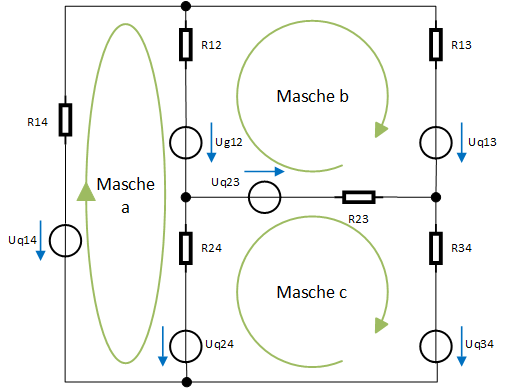
\includegraphics[width=0.7\textwidth]{Bruckenschaltung_mit_Maschen.png}
  \caption{Brückenschaltung mit Maschen}
  \label{fig:brueckenschaltung_maschen}
\end{figure}

Zur Maschenstromanalyse werden zunächst linear unabhängige Maschen aufgestellt. Im nächsten Schritt sind die Spannungssummen zu bilden, die nach dem 2. Kirchhoffschen Gesetz (siehe \ref{sec:kirch_2}) Null ergeben müssen.
  \begin{align}
    &\text{Masche a: }&-U_{q14} &+ U_{q12} &+ U_{q24} &+ (I_a - I_b)R_{12} &+ (I_a - I_c)R_{24} &+ R_{14} I_a &= 0 \nonumber \\
    &\text{Masche b: }&-U_{q12} &+ U_{q13} &- U_{q23} &+ (I_b - I_c)R_{23} &+ (I_b - Ia)R_{12} &+ I_b R_{13}  &= 0 \nonumber \\
    &\text{Masche c: }&-U_{q24} &+ U_{g23} &+ U_{q34} &+ (I_c - I_a)R_{24} &+ (I_c - I_b)R_{23} &+ I_c R_{34} &= 0
    \nonumber \\
  \end{align}
  Aus diesen so erhaltenen Maschengleichungen wird nun ein LGS aufgebaut:
  \begin{equation}
  \begin{tabularx}{14.7cm}{l|c c c | c}
    \textbf{Masche} & $I_a$ & $I_b$ & $I_c$ & \textbf{Quellen} \\ \hline
    \textbf{a: } & $R_{14}+R_{12}+R_{24}$ & $-R_{12}$ & $-R_{24}$ & $U_{q14} - U_{q12} - U_{q24}$ \\
    \textbf{b: } & $-R_{12}$ & $R_{12}+R_{13}+R_{23}$ & $-R_{23}$ & $U_{q12} - U_{q23} + U_{q13}$ \\
    \textbf{c: } & $-R_{24}$ & $-R_{23}$ & $R_{23}+R_{24}+R_{34}$ & $U_{q24} - U_{q23} - U_{q34}$ \\ 
    \multicolumn{5}{c}{$\;$}\\
  \end{tabularx}
  \end{equation}
  
  Dies lässt sich als Matrix einfacher darstellen:
  \begin{align}
    \left(
      \begin{array}{c c c}
      R_{14}+R_{12}+R_{24} & -R_{12} & -R_{24} \\
      -R_{12} & R_{12}+R_{13}+R_{23} & -R_{23} \\
      -R_{24} & -R_{23} & R_{23}+R_{24}+R_{34} \\
      \end{array}
    \right) \cdot \vecT{I_a \\ I_b \\ I_c} \nonumber \\
    = \vecT{U_{q14} - U_{q12} - U_{q24} \\ U_{q12} - U_{q23} + U_{q13} \\U_{q24} - U_{q23} - U_{q34}}
  \end{align}
  
  Diese Matrix lässt sich nun am einfachsten mit der Cramerschen Regel lösen. Da es sich um eine $3\times 3$ Matrix handelt, kann bequem mit der Sarruschen Regel gearbeitet werden.\newline
  Es gilt zunächst die Cramersche Regel:
  \begin{align}
    I_a = \frac{\det D_a}{\det D} \qquad \qquad I_b = \frac{\det D_b}{\det D} \qquad \qquad I_c = \frac{\det D_c}{\det D}
  \end{align}
  Die Determinanten werden über die Sarrussche Regel bestimmt:
  \begin{align}
    \det X &= \left|
      \begin{array}{c c c}
      X_{aa} & X_{ab} & X_{ac}\\
      X_{ba} & X_{bb} & X_{bc}\\
      X_{ca} & X_{cb} & X_{cc}\\
      \end{array}
    \right|    
    = \left|
      \begin{array}{c c c}
      \colGreen{X_{aa}} & \colGreen{X_{ab}} & \colGreen{X}_{\colBlue{ac}}\\
      X_{ba} & \colGreen{X}_{\colBlue{bb}} & \colGreen{X}_{\colBlue{bc}}\\
      \colBlue{X_{ca}} & \colBlue{X_{cb}} & \colGreen{X}_{\colBlue{cc}}\\
      \end{array}
    \right| 
    \begin{array}{c c}
      \colBlue{X_{aa}} & \colBlue{X_{ab}}\\
      \colGreen{X}_{\colBlue{ba}} & X_{bb}\\
      \colGreen{X_{ca}} & \colGreen{X_{cb}}\\
    \end{array} \nonumber \\
    \nonumber \\
    &\Rightarrow \det X =   \colGreen{X_{aa}} \colGreen{X_{bb}} \colGreen{X_{cc}} 
      + \colGreen{X_{ab}}   \colGreen{X_{bc}} \colGreen{X_{ca}}
      + \colGreen{X_{ac}}   \colGreen{X_{ba}} \colGreen{X_{cb}} \nonumber \\
      &\qquad \qquad \qquad- \colBlue{X_{ca}}    \colBlue{X_{bb}}  \colBlue{X_{ac}} 
      - \colBlue{X_{cb}}    \colBlue{X_{bc}}  \colBlue{X_{aa}}
      - \colBlue{X_{cc}}    \colBlue{X_{ba}}  \colBlue{X_{ab}}
  \end{align}
  
  Für die Berechnung der $Determinanten$ $D_a$, $D_b$ und $D_c$ wird nach der Cramerschen Regel jeweils die Spalte in der Matrix mit dem gesuchten Strom durch die Quellenspalte ausgetauscht.
  
  Allgemein gilt also:
  \begin{flalign}
  &X = \left(
    \begin{array}{c c c}
    X_{aa} & X_{ab} & X_{ac}\\
    X_{ba} & X_{bb} & X_{bc}\\
    X_{ca} & X_{cb} & X_{cc}\\
    \end{array}
  \right) \cdot \vecT{I_a \\ I_b \\ I_c} = \vecT{Y_a \\ Y_b \\ Y_c}  \nonumber \\
  \nonumber \\
  &\Rightarrow \det X_a = 
  \left|
    \begin{array}{c c c}
    Y_a & X_{ab} & X_{ac}\\
    Y_b & X_{bb} & X_{bc}\\
    Y_c & X_{cb} & X_{cc}\\
    \end{array}        
  \right|& \nonumber \\ 
  &= \colGreen{Y_a X_{bb} X_{cc}} + \colGreen{X_{ab}X_{bc}Y_c} + \colGreen{X_{ac} Y_b X_{cb}} - \colBlue{X_{ac} X_{bb} Y_c} - \colBlue{Y_a X_{bc} X_{cb}} - \colBlue{X_{ab} Y_b X_{cc}}& \\
  &\Rightarrow \det X_b = 
  \left|
    \begin{array}{c c c}
    X_{aa} & Y_a & X_{ac}\\
    X_{ba} & Y_b & X_{bc}\\
    X_{ca} & Y_c & X_{cc}\\
    \end{array}        
  \right|& \nonumber \\ 
  &= \colGreen{X_{aa} Y_b X_{cc}} + \colGreen{Y_a X_{bc} X_{ca}} + \colGreen{X_{ac} X_{ba} Y_c} - \colBlue{X_{ac} Y_b X_{ca}} - \colBlue{X_{aa} X_{bc} Y_c} - \colBlue{Y_a X_{ba} X_{cc}}& \\ 
  &\Rightarrow \det X_c = 
  \left|
    \begin{array}{c c c}
    X_{aa} & X_{ab} & Y_a\\
    X_{ba} & X_{bb} & Y_b\\
    X_{ca} & X_{cb} & Y_c\\
    \end{array}        
  \right|& \nonumber \\  
  &= \colGreen{X_{aa} X_{bb} Y_c} + \colGreen{X_{ab} Y_b X_{ca}} + \colGreen{Y_a X_{ba} X_{cb}} - \colBlue{Y_a X_{bb} X_{ca}} - \colBlue{X_{aa} Y_b X_{cb}} - \colBlue{X_{ab}X_{ba} Y_c}&\\
  \nonumber  \\
  %
  &\text{Somit ergibt sich für die einzelnen Ströme:}& \nonumber \\
  %
  \nonumber \\
    &I_a = \frac{\det D_a}{\det D} = \frac{
    \left|
    \begin{array}{c c c}
    Y_a & X_{ab} & X_{ac}\\
    Y_b & X_{bb} & X_{bc}\\
    Y_c & X_{cb} & X_{cc}\\
    \end{array}        
  \right|}{
    \left|
    \begin{array}{c c c}
    X_{aa} & X_{ab} & X_{ac}\\
    X_{ba} & X_{bb} & X_{bc}\\
    X_{ca} & X_{cb} & X_{cc}\\
    \end{array}
    \right|
  }& \nonumber \\
  &= \frac{
    Y_a(X_{bb} X_{cc} - X_{bc}X_{cb}) + Y_b(X_{ac} X_{cb} - X_{ab} X_{cc}) 
  + Y_c(X_{ab} X_{bc} - X_{ac} X_{bb})}{
     X_{aa} X_{bb} X_{cc} + X_{ab} X_{bc} X_{ca} + X_{ac} X_{ba} X_{cb} 
  - X_{ca} X_{bb} X_{ac} - X_{cb} X_{bc} X_{aa} - X_{cc}X_{ba} X_{ab}}& \nonumber \\
  \\  
  %      
  &I_b = \frac{\det D_b}{\det D} = \frac{
    \left|
    \begin{array}{c c c}
    X_{aa} & Y_a & X_{ac}\\
    X_{ba} & Y_b & X_{bc}\\
    X_{ca} & Y_c & X_{cc}\\
    \end{array}        
  \right|}{
    \left|
    \begin{array}{c c c}
    X_{aa} & X_{ab} & X_{ac}\\
    X_{ba} & X_{bb} & X_{bc}\\
    X_{ca} & X_{cb} & X_{cc}\\
    \end{array}
    \right|
  }& \nonumber \\
  &= \frac{
    Y_a(X_{bc} X_{ca} - X_{ba}X_{cc}) + Y_b(X_{aa} X_{cc} - X_{ac} X_{ca}) 
  + Y_c(X_{ac} X_{ba} - X_{aa} X_{bc})}{
     X_{aa} X_{bb} X_{cc} + X_{ab} X_{bc} X_{ca} + X_{ac} X_{ba} X_{cb} 
  - X_{ca} X_{bb} X_{ac} - X_{cb} X_{bc} X_{aa} - X_{cc}X_{ba} X_{ab}}& \nonumber \\
  \end{flalign}
  
  \begin{flalign}      
  &I_c = \frac{\det D_c}{\det D} = \frac{
    \left|
    \begin{array}{c c c}
    X_{aa} & X_{ab} & Y_a\\
    X_{ba} & X_{bb} & Y_b\\
    X_{ca} & X_{cb} & Y_c\\
    \end{array}        
  \right|}{
    \left|
    \begin{array}{c c c}
    X_{aa} & X_{ab} & X_{ac}\\
    X_{ba} & X_{bb} & X_{bc}\\
    X_{ca} & X_{cb} & X_{cc}\\
    \end{array}
    \right|
  }& \nonumber \\
  &= \frac{
    Y_a(X_{ba} X_{cb} - X_{bb}X_{ca}) + Y_b(X_{ab} X_{ca} - X_{aa} X_{cb}) 
  + Y_c(X_{aa} X_{bb} - X_{ab} X_{ba})}{
     X_{aa} X_{bb} X_{cc} + X_{ab} X_{bc} X_{ca} + X_{ac} X_{ba} X_{cb} 
  - X_{ca} X_{bb} X_{ac} - X_{cb} X_{bc} X_{aa} - X_{cc}X_{ba} X_{ab}}& \nonumber\\
  \end{flalign}
  Nach Einsetzen der entsprechenden Werte erhält man somit die Lösungen für die einzelnen Maschenströme.
  \subsection{Knotenspannungsanalyse} \label{sec:knotenspann}
  Bei der Knotenspannungsanalyse(Knotenpotenzialverfahren) wird jedem Knoten $i$ ein Potential $\varphi_i$ gegenüber einem Bezugspotential (in der Regel Masse) zugeordnet. Bei der Knotenspannungsanalyse werden entsprechend die Kotenpotentiale berechnet. Aus der Differenz der Potentiale lässt sich so die Spannung zwischen zwei Knoten bestimmen. Dieses Verfahren eignet sich besonders für die Betrachtung von idealen Stromquellen. Sind Spannungsquellen vorhanden, sollten diese durch Einführung eines endlichen Innenwiderstandes $R_i$ dann in ideale Stromquellen umformuliert werden. Bei der endgültigen Lösung muss dann allerdings zwingend $R_i \rightarrow 0$ beachtet werden.
  \begin{itemize}
    \item $I_{qkl}$ ist die Summe aller Stromquellen zwischen den Knoten $k$ und $l$.
    \item Es ergeben sich bei insgesamt $n$ Knoten insgesamt $n-1$ unabhängige Knotengleichungen. 
  \end{itemize}
  Allgemein ergibt sich damit:
 \begin{equation}
  \begin{tabularx}{14.7cm}{l|c c c c | c}
    \textbf{Knoten} & $\varphi_1$ & $\varphi_2$ & $...$ & $\varphi_{n-1}$ &  \textbf{Quellenstrom in Knoten} \\ \hline
    \textbf{1: }    & $G_{ii}$    & $-G_{12}$   & $...$ & $-G_{1,n-1}$    & $I_{q,1}$ \\
    \textbf{2: }    & $-G_{21}$   & $G_{22}$    & $...$ & $...$           & $I_{q,2}$ \\
    $.$             & $...$       & $...$       & $...$ & $...$           & $...$      \\    
    \textbf{n-1: }  & $...$       & $...$       & $...$ & $G_{n-1,n-1}$   & $I_{q,n-1}$ \\ 
    \multicolumn{6}{c}{$\;$}\\
  \end{tabularx}
  \end{equation}
  
  Wobei gilt:
  \begin{itemize}
    \item $G_{ii}$ ist die Summe aller Leitwerte die mit dem Knoten $i$ direkt verbunden sind und positiv ins Schema einzutragen.
    \item $G_{ij}$ ist die Summe aller Leitwerte zwischen den Knoten $i$ und $j$ und negativ ins Schema einzutragen.
    \item $I_{qi}$ ist die Summe aller durch Stromquellen in den Knoten $i$ fließenden Ströme.
    \item Wurde als Bezugsknoten $\varphi_n = 0$ gewählt gilt für die Knotenspannungen: $U_{kn} = \varphi_k - \varphi n = \varphi_k$.
  \end{itemize}
  %Bruckenschaltung_mit_Knotenspannungsanalyse.png
  \begin{figure}[htbp] 
	  \centering
	  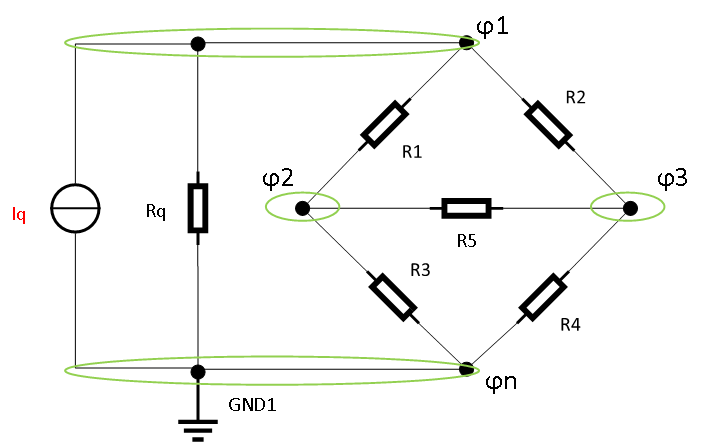
\includegraphics[width=0.7\textwidth]{Bruckenschaltung_mit_Knotenspannungsanalyse.png}
	  \caption{Brückenschaltung mit Knoten}
	  \label{fig:brueckenschaltung_knoten}
  \end{figure}
  
  Diese Schaltung lässt sich einfach mit dem oben beschriebenen Schema als LGS formulieren:
  \begin{equation}
  \begin{tabularx}{14.7cm}{l|c c c c | c}
    \textbf{Knoten} & $\varphi_1$ & $\varphi_2$ & $\varphi_3$ &  \textbf{Quellen} \\ \hline
    \textbf{1: }    & $\frac{1}{R_1} + \frac{1}{R_2} + \frac{1}{R_q}$    & $-\frac{1}{R_1}$    & $-\frac{1}{R_2}$           & $I_q$ \\
    \textbf{2: }    & $-\frac{1}{R_1}$   & $\frac{1}{R_1} + \frac{1}{R_3} + \frac{1}{R_5}$    & $-\frac{1}{R_5}$           & $0$ \\
    \textbf{3: }    & $-\frac{1}{R_2}$    & $-\frac{1}{R_5}$             & $\frac{1}{R_2} + \frac{1}{R_4} + \frac{1}{R_5}$    & $0$ \\ 
    \multicolumn{6}{c}{$\;$}\\
  \end{tabularx}
  \end{equation}
  
  Bzw. als Matrix:
  \begin{align}
    \left(
      \begin{array}{c c c}
      \frac{1}{R_1} + \frac{1}{R_2} + \frac{1}{R_q} & -\frac{1}{R_1}                                & -\frac{1}{R_2} \\
      -\frac{1}{R_1}                                & \frac{1}{R_1} + \frac{1}{R_3} + \frac{1}{R_5} & -\frac{1}{R_5} \\
      -\frac{1}{R_2}                                & -\frac{1}{R_5}                                & \frac{1}{R_2} + \frac{1}{R_4} + \frac{1}{R_5} \\
      \end{array}
    \right) \cdot \vecT{\varphi_1 \\ \varphi_2 \\ \varphi_3} \nonumber \\
    = \vecT{I_q \\ 0 \\0}
  \end{align}
  
  \subsection{Superpositionsprinzip nach Helmholtz}
  Bei Netzwerken mit ausschließlich linearen Netzwerken kann die Berechnung vereinfacht werden, in dem die Spannungsquellen/Stromquellen einzeln betrachtet werden, d.h. es werden immer alle Quellen bis auf eine \dq ausgeschaltet \dq betrachtet. Hierbei gilt für die nichtaktiven Quellen:
  \begin{itemize}
    \item Ideale Spannungsquelle: Kurzschließen
    \item Ideale Stromquelle    : \dq Offen lassen \dq, d.h. Leerlauf  
  \end{itemize}
  Es werden zunächste alle einzelnen Ströme für Quelle $1$: $I_1', I_2', ..., I_n'$, Quelle $2$:$I_1'', I_2'', ..., I_n''$, ... bis Quelle $n$  im Zustand mit deaktivierten Quellen berechnet. Die Gesamtsröme ergeben sich dann aus 
  \begin{equation}
    I_i = I_i' + I_i'' + ... + i_i^{(n)}
  \end{equation}
  
  \subsection{Ersatzquellenverfahren}
  Häufig zielführend ist es Ersatzspannungs- bzw. Ersatzstromquelle zu definieren.
\newpage
\section{\underline{Anhänge}}
\subsection{Abkürzungen/Formelzeichen}
\renewcommand{\arraystretch}{1.5}

\begin{longtable} {|p{2cm}|p{3cm}|p{9cm}|} \hline
% Definition des Tabellenkopfes auf der ersten Seite
%Spaltenbezeichnungen
\textbf{Zeichen} & \textbf{Einheit} & \textbf{Bedeutung} \\
\hline
\endfirsthead % Erster Kopf zu Ende
% Definition des Tabellenkopfes auf den folgenden Seiten
\caption{Fortsetzung}\\ \hline
%Spaltenbezeichnungen
\textbf{Zeichen} & \textbf{Einheit} & \textbf{Bedeutung} \\
\hline
\endhead % Zweiter Kopf ist zu Ende
\multicolumn{3}{r}{Fortsetzung auf Folgeseite}\\
\endfoot
\hline
%\multicolumn{3}{r}{Ende} \\
\endlastfoot

%a-g
$A$ & $m^2$ & Fläche \\ \hline
$a$ & $\frac{m}{s^2}$ & Beschleunigung \\ \hline
$b$ & $\frac{cm^2}{Vs}$ & Ladungsträgerbeweglichkeit \\ \hline
$d$ & $m$ & Dicke \\ \hline
$e$ & $C$ & Elementarladung \\ \hline
$E$ & $\frac{N}{C} = \frac{VAs}{mAs} = \frac{V}{m}$ & Elektrische Feldstärke \\ \hline
$\vec{F}$ & $N = \frac{kgm}{s^2}$ & Kraft \\ \hline
$G$ & $\frac{A}{V} = \frac{1}{\Omega} = S$ & Leitwert \\ \hline

%h-n
$i$ & $A$ & Elektrischer Strom \\ \hline
$j$ & $\frac{A}{m2}$ & Elektrische Stromdichte \\ \hline
$l$ & $m$ & Länge \\ \hline

%m-u
$q$ & $C$ & Probeladung (in der Regel = $e$) \\ \hline
$\vec{r}$ & $m$ & Weg \\ \hline
$r$ & $\Omega$ & Differentieller Widerstand \\ \hline
$R$ & $\Omega$ & Widerstand \\ \hline
$R_F$ & $\frac{\Omega}{square}$ & Flächenwiderstand \\ \hline 
$U$ & $V$ & Elektrische Spannung \\ \hline
$U_g$ & $V$ & Gesamtspannung \\ \hline
 
%v-z
$v$ & $\frac{m}{s}$ & Geschwindigkeit \\ \hline
$v_D$ & $\frac{m}{s}$ & Driftgeschwindigkeit \\ \hline
$w$ & $m$ & Weite bzw. Breite  \\ \hline
$W$ & $Ws = J = \frac{kgm^2}{s^2}$ & Arbeit bzw. Energie \\ \hline

%griechisch
$\alpha$ & $\frac{1}{^{\circ} C}$ & Temperturkoeffizient des Ohmwiderstandes \\ \hline
$\rho$ & $\frac{V cm}{A} = \Omega  cm$ & Spezifischer Widerstand \\ \hline
$\kappa$ & $\frac{1}{\Omega cm} = \frac{S}{cm}$ & Spezifische Leitfähigkeit \\ \hline
$\varepsilon_0$ & $\frac{As}{Vm}$ & Dielektrizitätskonstante im Vakuum \\ \hline
$\varphi$ & $V$ & Elektrisches Potential \\ \hline
$\tau$ & $s$ & Stoßzeit \\ \hline

%Sonderzeichen
\end{longtable}
\renewcommand{\arraystretch}{1}
\subsection{Formelverzeichnis}


\bibliography{lit}

\end{document}
